\section{GNU Radio setup, simulation results and comments}

\subsection{AM Communication}

    - arquitetura
    - tone test 
    - teste com musica

\subsection{Digital Modulation}

Explicar:
    Symbol Mapping, Constellation Diagrams, and Gray Coding
    Falar to piloto algures


\label{ssec:modulations}
For this labwork, different mapping strategies were used, QPSK and 16-QAM.

\textbf{QPSK} places four equally spaced points on the unit circle:
\[
s_k = e^{j\frac{\pi}{2}\left(k+\tfrac12\right)}, \qquad k\in\{0,1,2,3\}.
\]

Figure \ref{fig:QPSK_const}, shows the mapping in the cartesian plane.


The mapper groups the encoded bit stream into two-bit tuples $(b_1,b_0)$, converts each tuple to an integer index $(k =2b_1+b_0)$ and outputs \(s_k\).

The theoretical bit-error probability for QPSK in an AWGN channel is given by Equation \ref{eq:probErrQPSK}.
\begin{equation}
  P_b^{\text{QPSK}} = Q\left(\sqrt{2\frac{E_b}{N_0}}\right)\text{\cite{Work_TAC2025}}
  \label{eq:probErrQPSK}
\end{equation}

For \textbf{QPSK}, demodulation is performed by simply de-mapping the bit values.


A square $4\times4$ 16-QAM constellation is used. What changes comparing to the previous mapping approach is the fact that the amplitude also changes and for this specific mapping the phase and amplitude will not change consistently. The symbol position in the cartesian frame will be:
\[
I,R \in \{\pm3,\;\pm1\}
\]

For \textbf{16-QAM} the theoretical \textbf{BER} for an AWGN channel with gray mapping is given by Equation \ref{eq:probErr16QAM}.

\begin{equation}
  P_b^{\text{16QAM}} \approx \frac{3}{4}\cdot Q\left(\sqrt{\frac{4}{5}\frac{E_b}{N_0}}\right)\text{\cite{Work_TAC2025}}
  \label{eq:probErr16QAM}
\end{equation}

%Because \textbf{16-QAM} is being compared to \textbf{QPSK}, the \textbf{SNR} must be consistent throughout both modulations, therefore every \textbf{16-QAM} symbol is divided by $\sqrt{10}$, normalizing the average symbol energy.

The constellation points are labelled with \emph{Gray coding}, thus every nearest neighbour differs in \emph{exactly one} bit, this will minimize \textbf{BER}, since the most likely symbol error produces only one wrong bit. Figure \ref{fig:16QAM_const}, shows how the codes are mapped.


\begin{comment}
    
\begin{figure}[H]
    \centering
    \includegraphics*[width=0.8\textwidth]{Images/Const_QPSK.png}
    \caption{QPSK Constellation}
    \label{fig:QPSK_const}
\end{figure}

\begin{figure}[H]
    \centering
    \includegraphics*[width=0.8\textwidth]{Images/Const_16QAM.png}
    \caption{16-QAM Constellation}
    \label{fig:16qam_const}
\end{figure}

\end{comment}

\begin{figure}[H]
    \centering
    \begin{subfigure}[t]{0.5\textwidth}
        \centering
        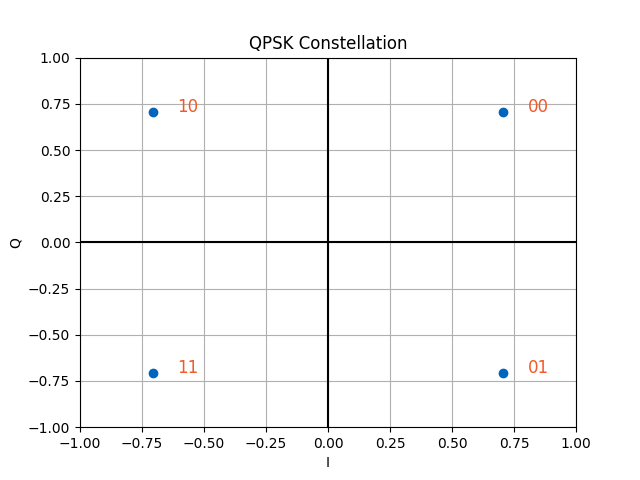
\includegraphics[width=\textwidth]{Images/Const_QPSK.png}
        \caption{QPSK Constellation.}
        \label{fig:QPSK_const}
    \end{subfigure}%
    \begin{subfigure}[t]{0.5\textwidth}
        \centering
        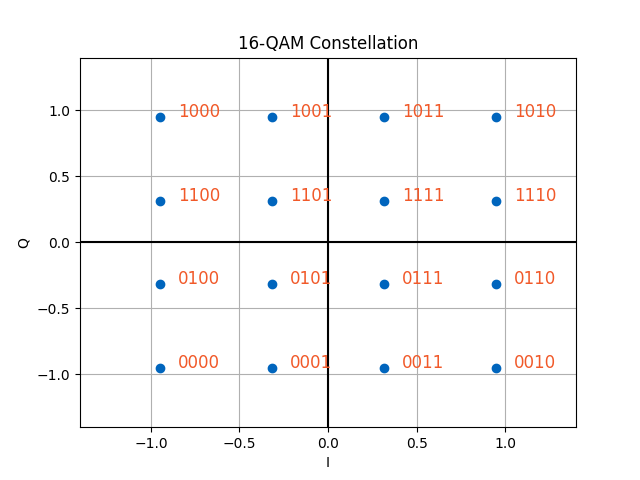
\includegraphics[width=\textwidth]{Images/Const_16QAM.png}
        \caption{16-QAM Constellation.}
        \label{fig:16QAM_const}
    \end{subfigure}
    \caption{Digital Modulation Constellations.}
    \label{fig:Const}
\end{figure}

\textcolor{red}{TODO: escrever os topicos}
condicoes:
    LP : Transition 500hz cutoff 40k
    SimbRate: 20k
    a3 emitter  = 0
    a3 receiver = 0
    no Bandpass

Dizer que bate certo com os valores teoricos e que 16 qam produz mais erros.

\begin{figure}[H]
    \centering
    \includegraphics*[width=0.8\textwidth]{Images/BER_SNR_a3_0.png}
    \caption{BER vs $E_b/N_0$}
    \label{fig:BER_SNR_a3_0}
\end{figure}